% Autor: Leonhard Segger, Alexander Neuwirth
% Datum: 2017-10-30
\documentclass[
	% Papierformat
	a4paper,
	% Schriftgröße (beliebige Größen mit „fontsize=Xpt“)
	12pt,
	% Schreibt die Papiergröße korrekt ins Ausgabedokument
	pagesize,
	% Sprache für z.B. Babel
	ngerman
]{scrartcl}

% Achtung: Die Reihenfolge der Pakete kann (leider) wichtig sein!
% Insbesondere sollten (so wie hier) babel, fontenc und inputenc (in dieser
% Reihenfolge) als Erstes und hyperref und cleveref (Reihenfolge auch hier
% beachten) als Letztes geladen werden!

% Silbentrennung etc.; Sprache wird durch Option bei \documentclass festgelegt
\usepackage{babel}
% Verwendung der Zeichentabelle T1 (Sonderzeichen etc.)
\usepackage[T1]{fontenc}
% Legt die Zeichenkodierung der Eingabedatei fest, z.B. UTF-8
\usepackage[utf8]{inputenc}
% Schriftart
\usepackage{lmodern}
% Zusätzliche Sonderzeichen
\usepackage{textcomp}

% Mathepaket (intlimits: Grenzen über/unter Integralzeichen)
\usepackage[intlimits]{amsmath}
% Ermöglicht die Nutzung von \SI{Zahl}{Einheit} u.a.
\usepackage{siunitx}
% Zum flexiblen Einbinden von Grafiken (\includegraphics)
\usepackage{graphicx}
% Abbildungen im Fließtext
\usepackage{wrapfig}
% Abbildungen nebeneinander (subfigure, subtable)
\usepackage{subcaption}
% Funktionen für Anführungszeichen
\usepackage{csquotes}
% Zitieren, Bibliographie
\usepackage{biblatex}

% Verlinkt Textstellen im PDF-Dokument
\usepackage[unicode]{hyperref}
% "Schlaue" Referenzen (nach hyperref laden!)
\usepackage{cleveref}
% Zur Darstellung von Webadressen
\usepackage{url}
%chemische Formeln
\usepackage[version=4]{mhchem}
% siunitx: Deutsche Ausgabe, Messfehler getrennt mit ± ausgeben
\usepackage{floatrow}
\floatsetup[table]{capposition=top}
\sisetup{
	locale=DE,
	separate-uncertainty
}
%\bibliography{6Mi_S2_25-10-2017_References}

\begin{document}
	
	\begin{titlepage}
		\centering
		{\scshape\LARGE Versuchsbericht zu \par}
		\vspace{1cm}
		{\scshape\huge M2 - Gekoppelte Pendel\par}
		\vspace{2.5cm}
		{\LARGE Gruppe 6Mi \par}
		\vspace{0.5cm}
		
		{\large Alexander Neuwirth (E-Mail: a\_neuw01@wwu.de) \par}
		{\large Leonhard Segger (E-Mail: l\_segg03@uni-muenster.de) \par}
		\vfill
		
		durchgeführt am 22.11.2017\par
		betreut von\par
		{\large Martin Körsgen}
		
		\vfill
		
		{\large \today\par}
	\end{titlepage}
	\tableofcontents
	\newpage
	
	\section{Kurzfassung}
	%TODO machen
	In diesem Versuch wurde das Verhalten zweier Pendel, die mittels einer Feder gekoppelt wurden, untersucht. Dazu sollte der Kopplungsgrad dynamisch sowie statisch bestimmt werden.
	Es wurde mit zwei verschieden starken Federn experimentiert.
	Zuletzt haben wir ein Doppelpendel beobachtet und dessen Bewegung mit der der gekoppelten Pendel verglichen.

	\section{Methoden}
	Der Versuch besteht aus zwei Pendeln die mittels verschieden starken Federn gekoppelt werden. Damit beide Pendeln mit der gleiche Eigenfrequenz schwingen, haben wir die Länge der Pendel so angepasst, dass sie auch nach ca. 20 Perioden ohne Kopplung synchron schwingen. Die Federn wurden \SI{10}{cm} über den Massen der Pendel befestigt. 
	
	Der Kopplungsgrad und die relative Frequenzaufspaltung wurde statisch sowie dynamisch bestimmt. Bei der statischen Messung wird ein Pendel ausgelenkt und die resultierende Auslenkung des anderen Pendels aufgenommen. Dynamisch ergibt sich der Kopplungsgrad aus den Schwingdauern der Grundschwingungen einer gleichsinnigen und gegensinnigen Bewegung. Eine gleichsinnige Bewegung wird erzeugt indem man beide Pendel in die gleiche Richtung um den gleiche Winkel auslenkt. Für eine gegensinnige Schwingung lenkt man die Pendel gleich weit in entgegengesetzte Richtungen aus.
	
	Experimentiert wurde mit einer Feder aus Kupfer und einer vermutlich aus Edelstahl bestehenden Feder.
	Zum Bestimmen der Schwingdauern wurde ein Ultraschall-Entfernungssensor verwendet, jedoch traten beim Testen der Messapperatur bei Sensorfrequenzen über \SI{50}{Hz} Softwareprobleme auf.

	Das Verhalten eines Doppelpendels wurde beobachtet mit verschiedenen initialen Auslenkungen und Geschwindigkeiten. 
	

	\section{Ergebnisse und Diskussion}
	In allen folgenden Abbildungen sind in Schwarz Entfernungsmessungspunkte des Ultraschallsensors mit \SI{50}{Hz}, sowie ein nicht linearer Fit in Rot aufgetragen.  Die Fit-Kurven wurden gemäß dem \enquote{Scaled Levenberg-Marquardt algorithm} erzeugt. Gemessen wurde immer über \SI{60}{} Sekunden. Lediglich zum Bestimmen der Schwebungsdauer wurde über \SI{120}{} Sekunden gemessen. %TODO Gleichung für Fit in Text aufnemen
	\subsection{Pendel ohne Kopplung}
	Die Schwingdauer eines einzelnen Pendels lässt sich am Parameter $b$ ablesen. Somit ist $T_0 =  \SI{2,477}{s}$.

	\begin{figure}[H]
		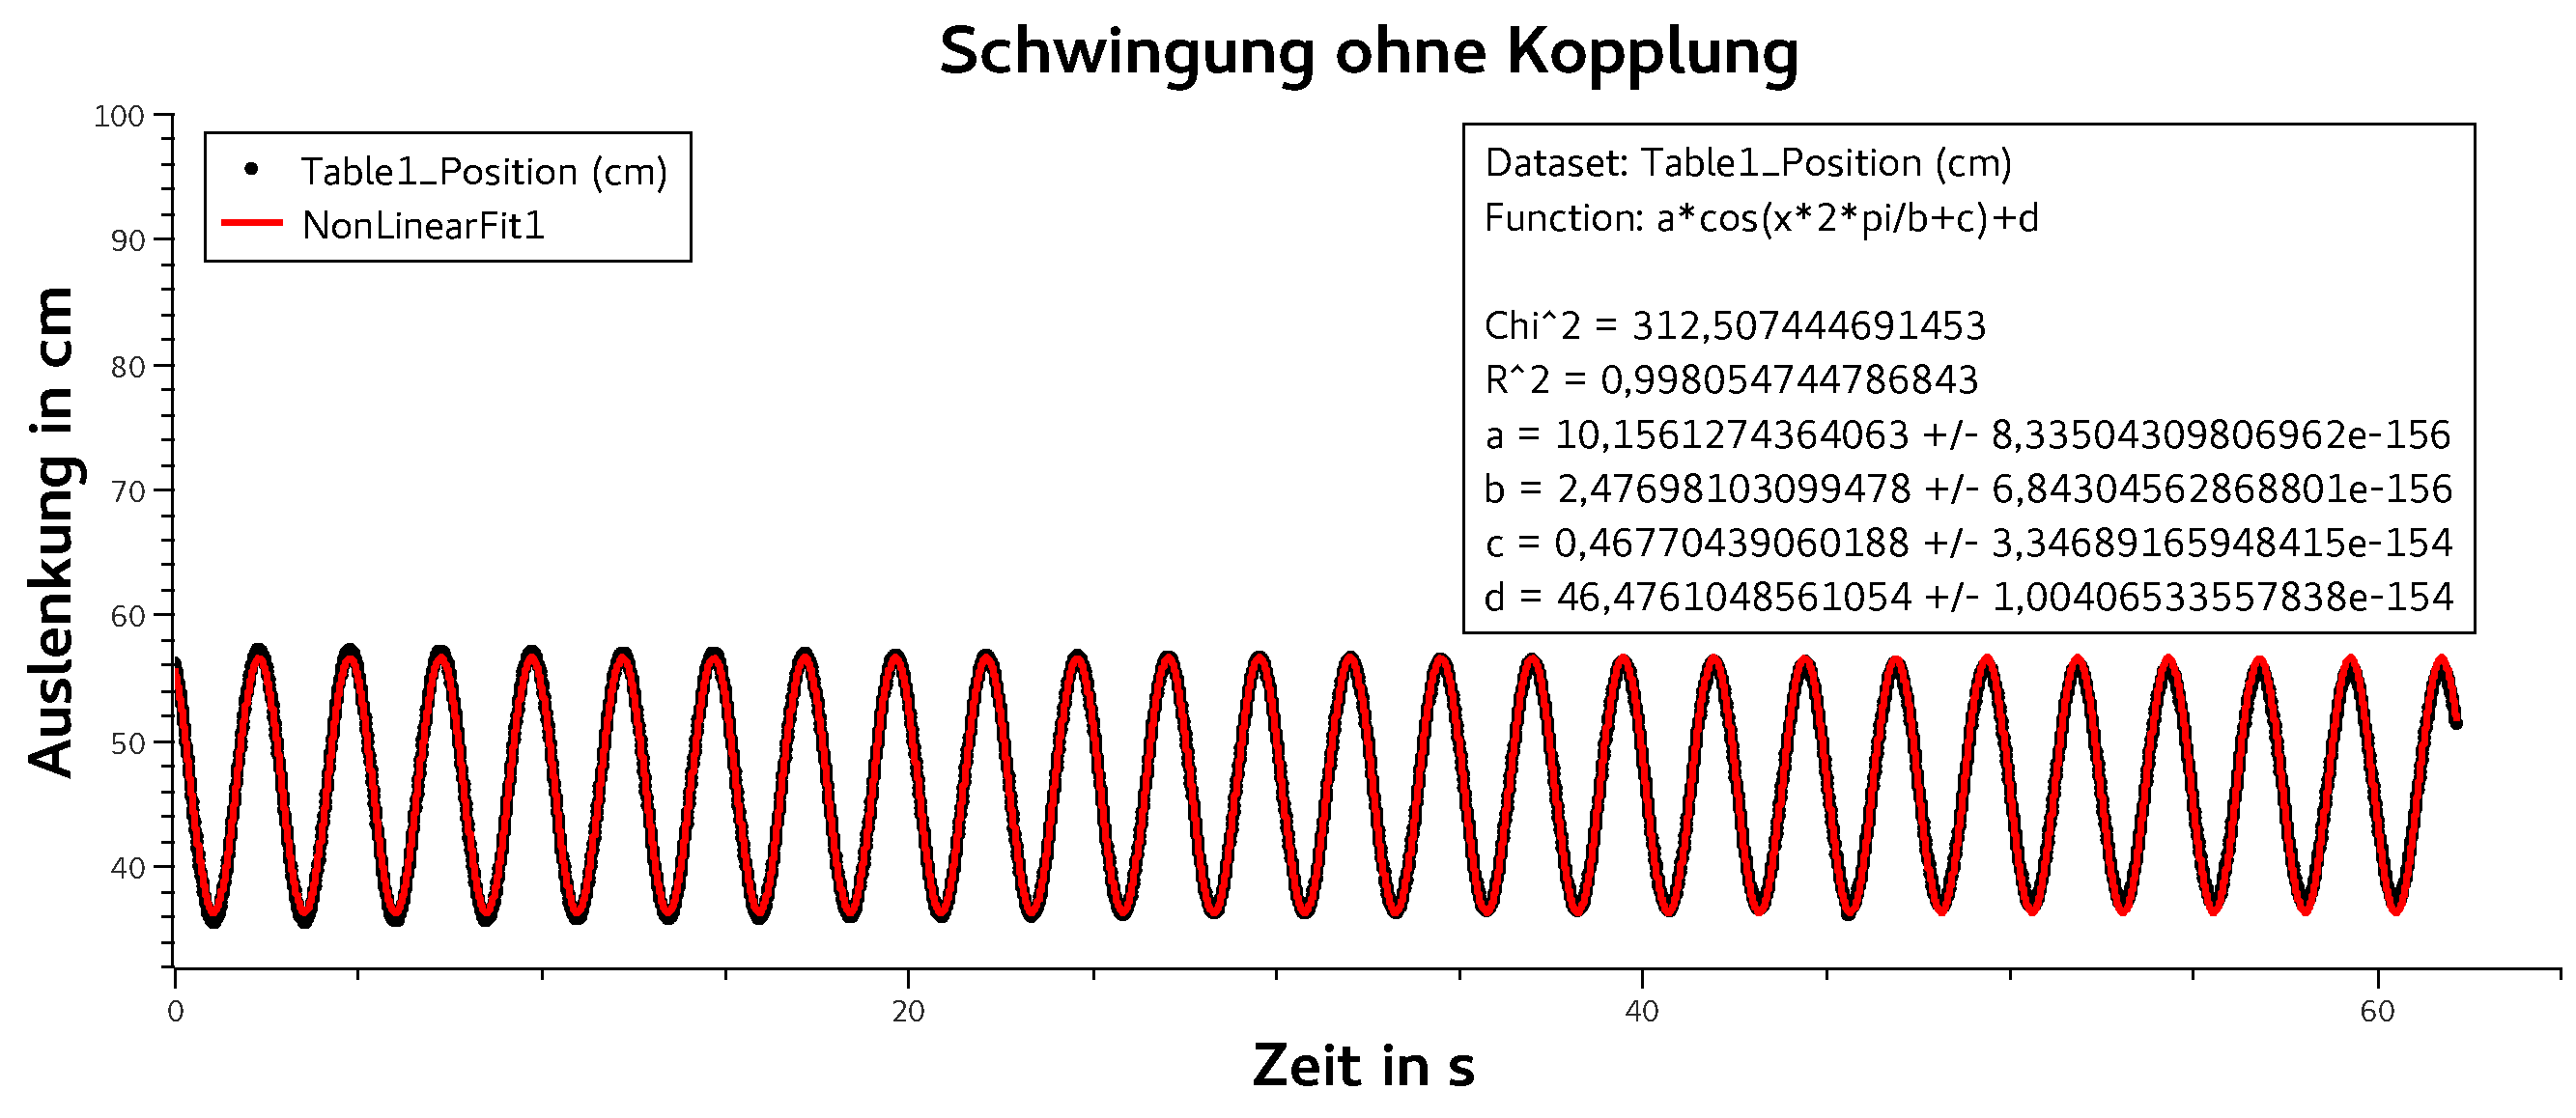
\includegraphics[width=1\textwidth]{SchwingungOhneKopplung}
		\centering
		\caption{Schwingung eines Fadenpendels.}
		\label{SchwingungOhneKopplung}
		\centering
	\end{figure}

	\subsection{Gekoppelte Pendel}
	\subsubsection{Statische Bestimmung des Kopplungsgrades}
	Die gegeben Formel für den Kopplungsgrad lautet:
	\begin{equation}
		k = \frac{x_2}{x_1}.
	\end{equation}
	Die Auslenkung der Pendel konnte bis auf $\Delta x = \pm \SI{0,1}{cm}$ genau bestimmt werden.
	Für die Unsicherheit ergibt sich also $u(x) = \frac{\SI{0,2}{cm}}{2\sqrt{3}} = \SI{0,058}{cm}$.
	\begin{equation}
		u(k) = \sqrt{\left(\frac{\partial k}{\partial x_1}u(x_1)\right)^2+\left(\frac{\partial k}{\partial x_2}u(x_2)\right)^2} = k u(x) \sqrt{\left(\frac{1}{x_1}\right)^2+\left(\frac{1}{x_2}\right)^2}
	\end{equation}
	\begin{table}[H]
	\centering
	\begin{tabular}{ l | c | c | c |}
		& Kupfer & Edelstahl  \\ \hline
		$x_1 $ &$\SI{9,8 \pm 0,058}{cm}$&$\SI{10,0 \pm 0,058}{cm}$\\  
		$x_2 $ &$\SI{1,9 \pm 0,058}{cm}$&$\SI{3,1 \pm 0,058}{cm}$\\  \hline\hline
		$k$  & $\SI{0,194 \pm 0,006}{}$ &  $\SI{0,310 \pm 0,006}{}$ \\ \hline
	\end{tabular}
	\caption{Messwerte beim Auslenken eines Pendels um $x_1$ und der resultierende Ausschlag des gekoppelten Pendels um $x_2$}
		\label{TabelleStatischKopplungsgrad}
	\end{table}

	\subsubsection{Gleichschwingung}

	\subsubsection*{Kupfer}
	Aus \cref{KupferGleichschwingung} lässt sich $T_\text{gl,Cu}$ aus den Parametern des Fits ablesen. Der Parameter $b$ ist die Schwingdauer und beträgt \SI{2,4645}{s}.
	\begin{figure}[H]
		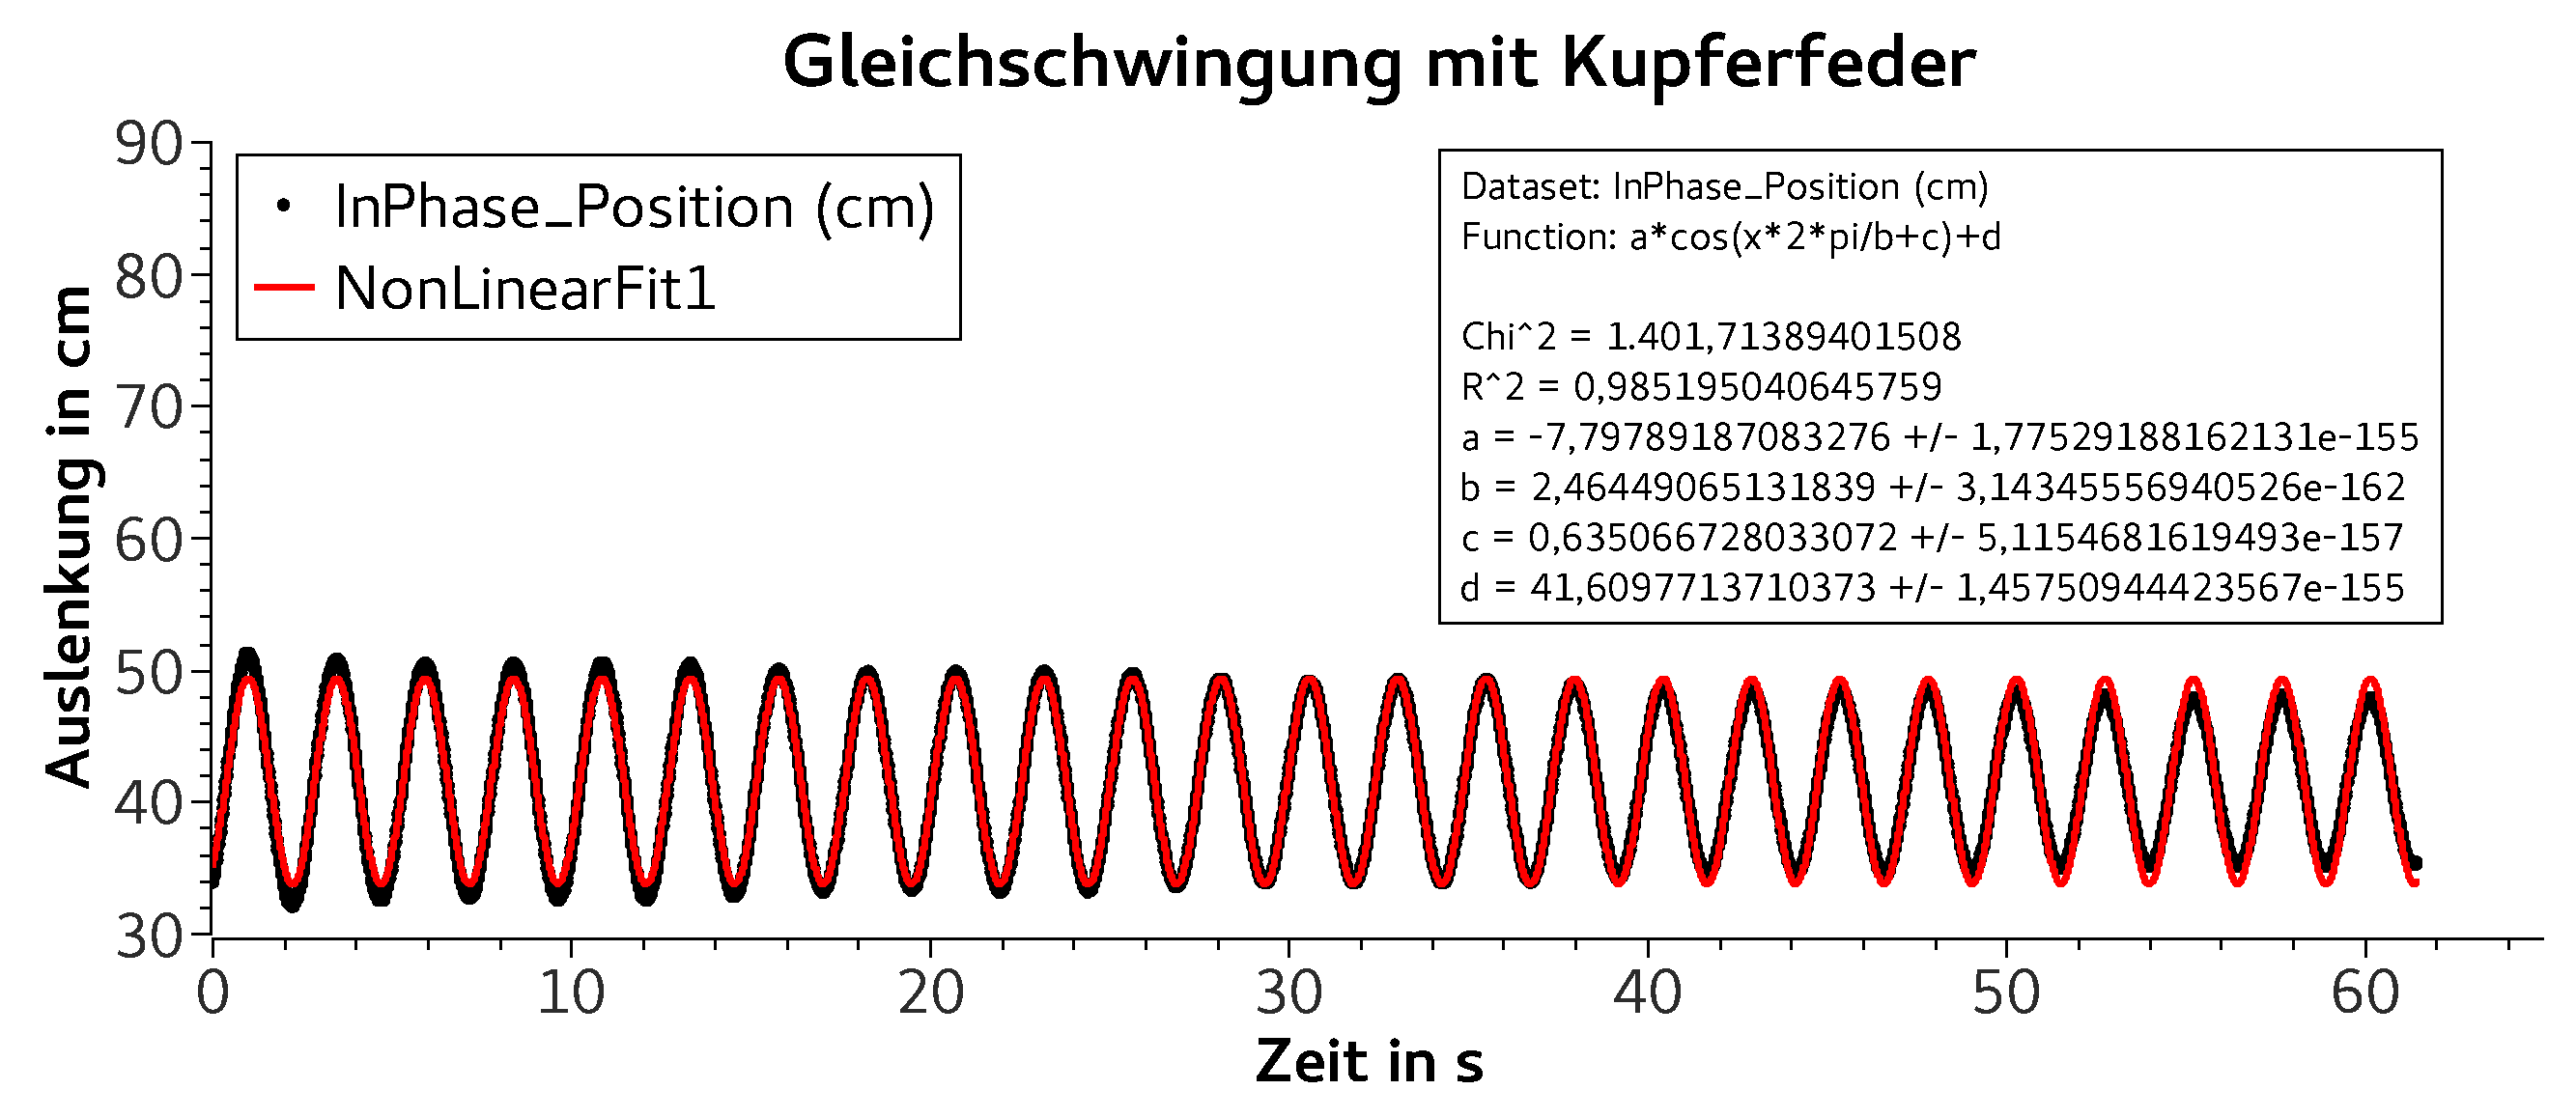
\includegraphics[width=1\textwidth]{KupferGleichschwingung}
		\centering
		\caption{Gleichschwingung mit Kupferfeder.}
		\label{KupferGleichschwingung}
		\centering
	\end{figure}

	\subsubsection*{Edelstahl}
	Aus \cref{EdelstahlGleichschwingung} lässt sich $T_\text{gl,St}$ aus den Parametern des Fits ablesen. Der Parameter $b$ ist die Schwingdauer und beträgt \SI{2,4437}{s}.
	\begin{figure}[H]
		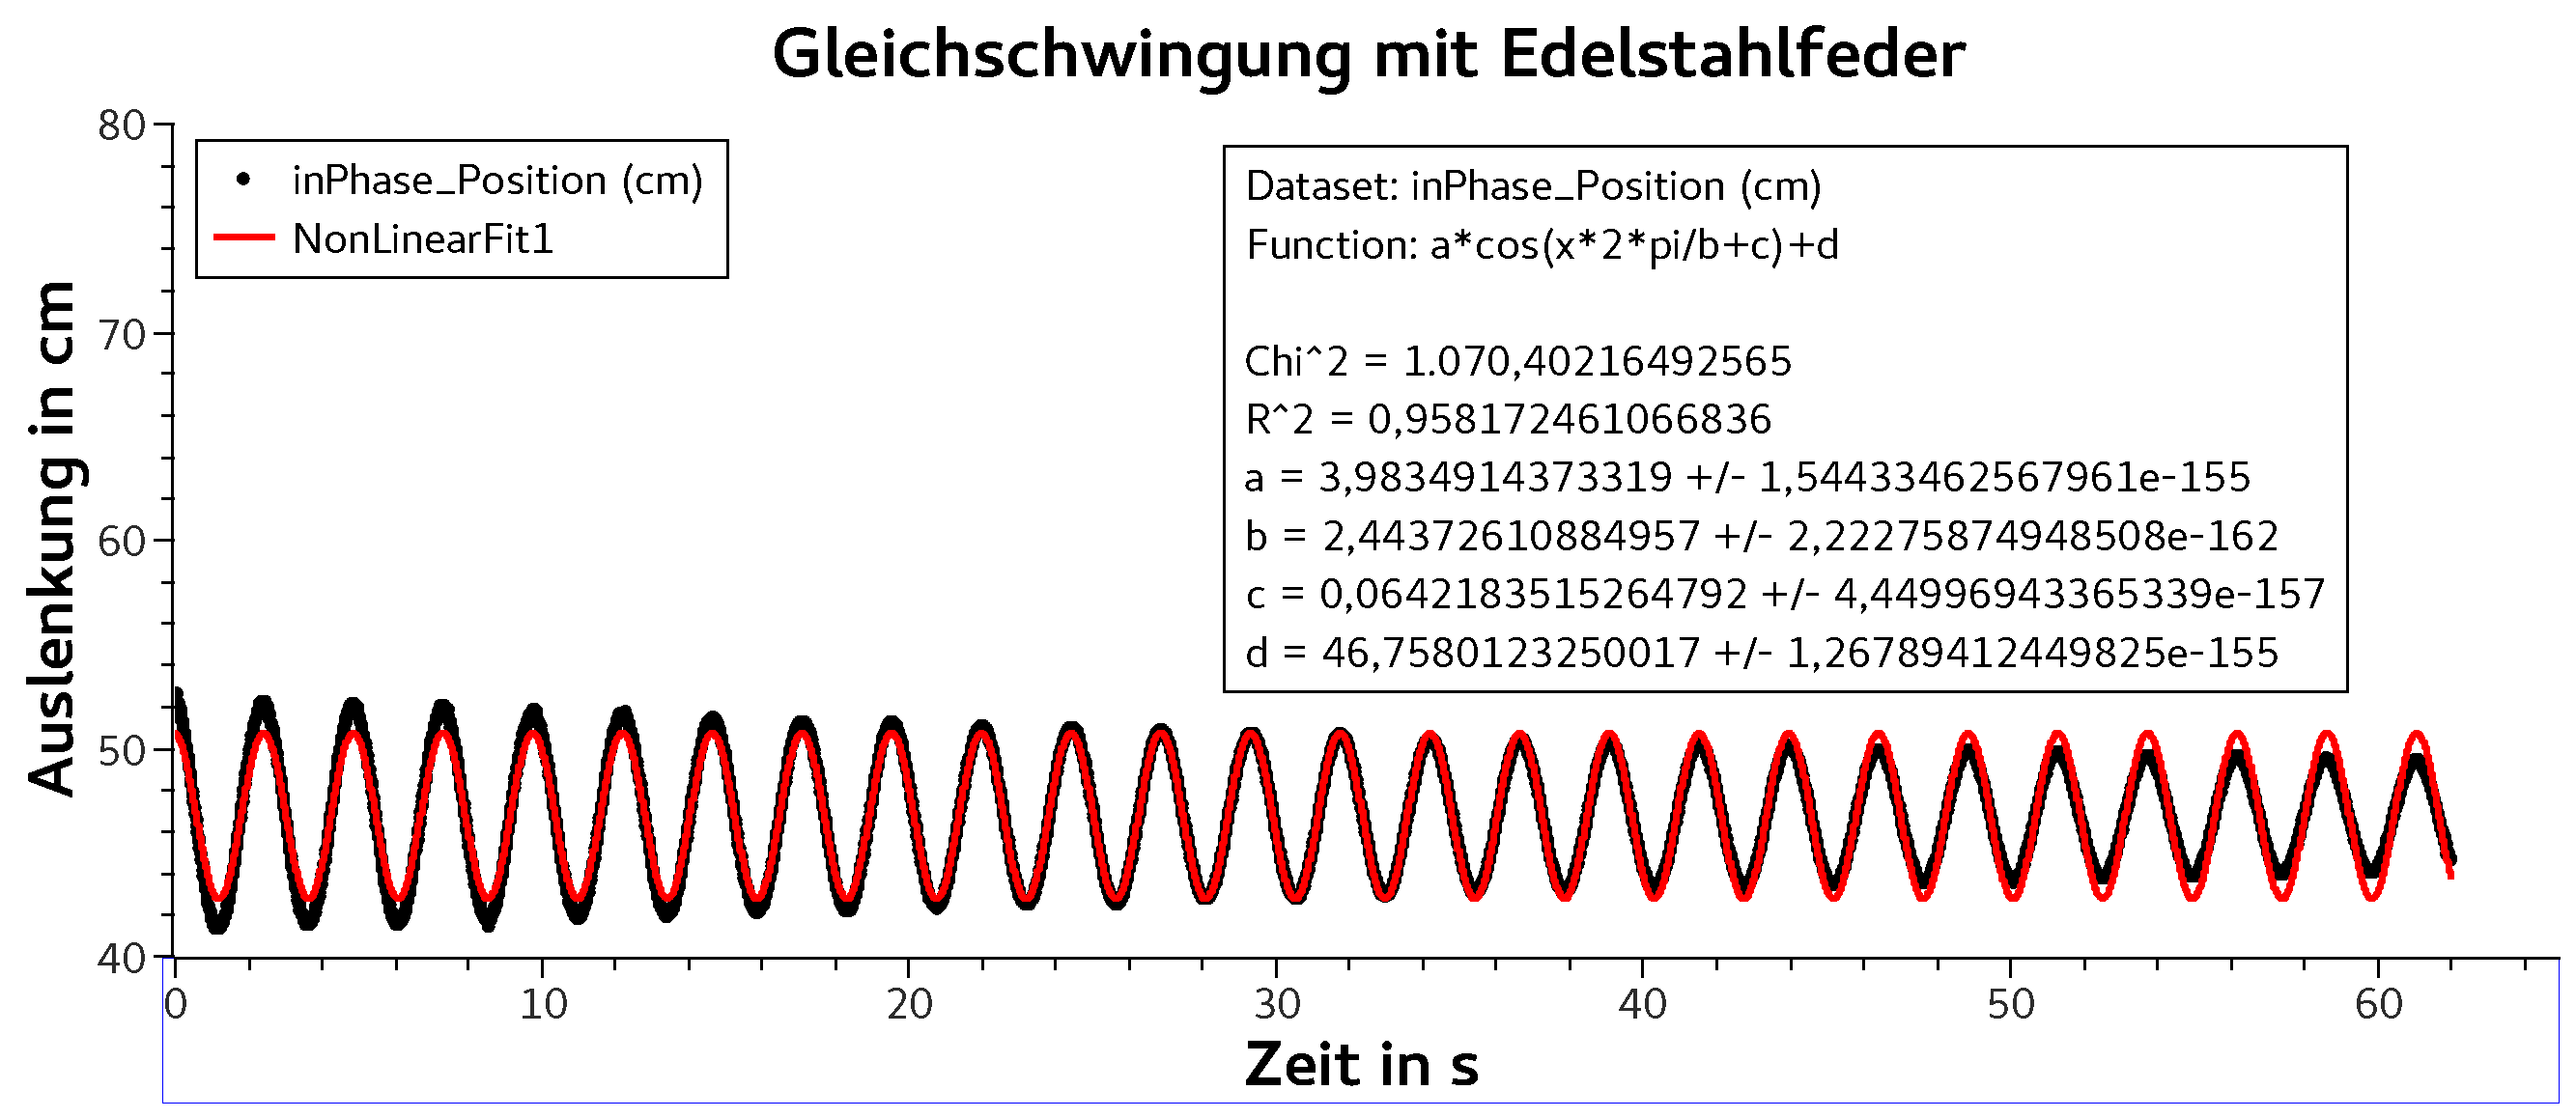
\includegraphics[width=1\textwidth]{EdelstahlGleichschwingung}
		\centering
		\caption{Gleichschwingung mit Edelstahlfeder.}
		\label{EdelstahlGleichschwingung}
		\centering
	\end{figure}


	\subsubsection{Gegenschwingung}

	\subsubsection*{Kupfer}
	Aus \cref{KupferGegenschwingung} lässt sich $T_\text{geg,Cu}$ aus den Parametern des Fits ablesen. Der Parameter $b$ ist die Schwingdauer und beträgt \SI{2,0381}{s}.
	\begin{figure}[H]
		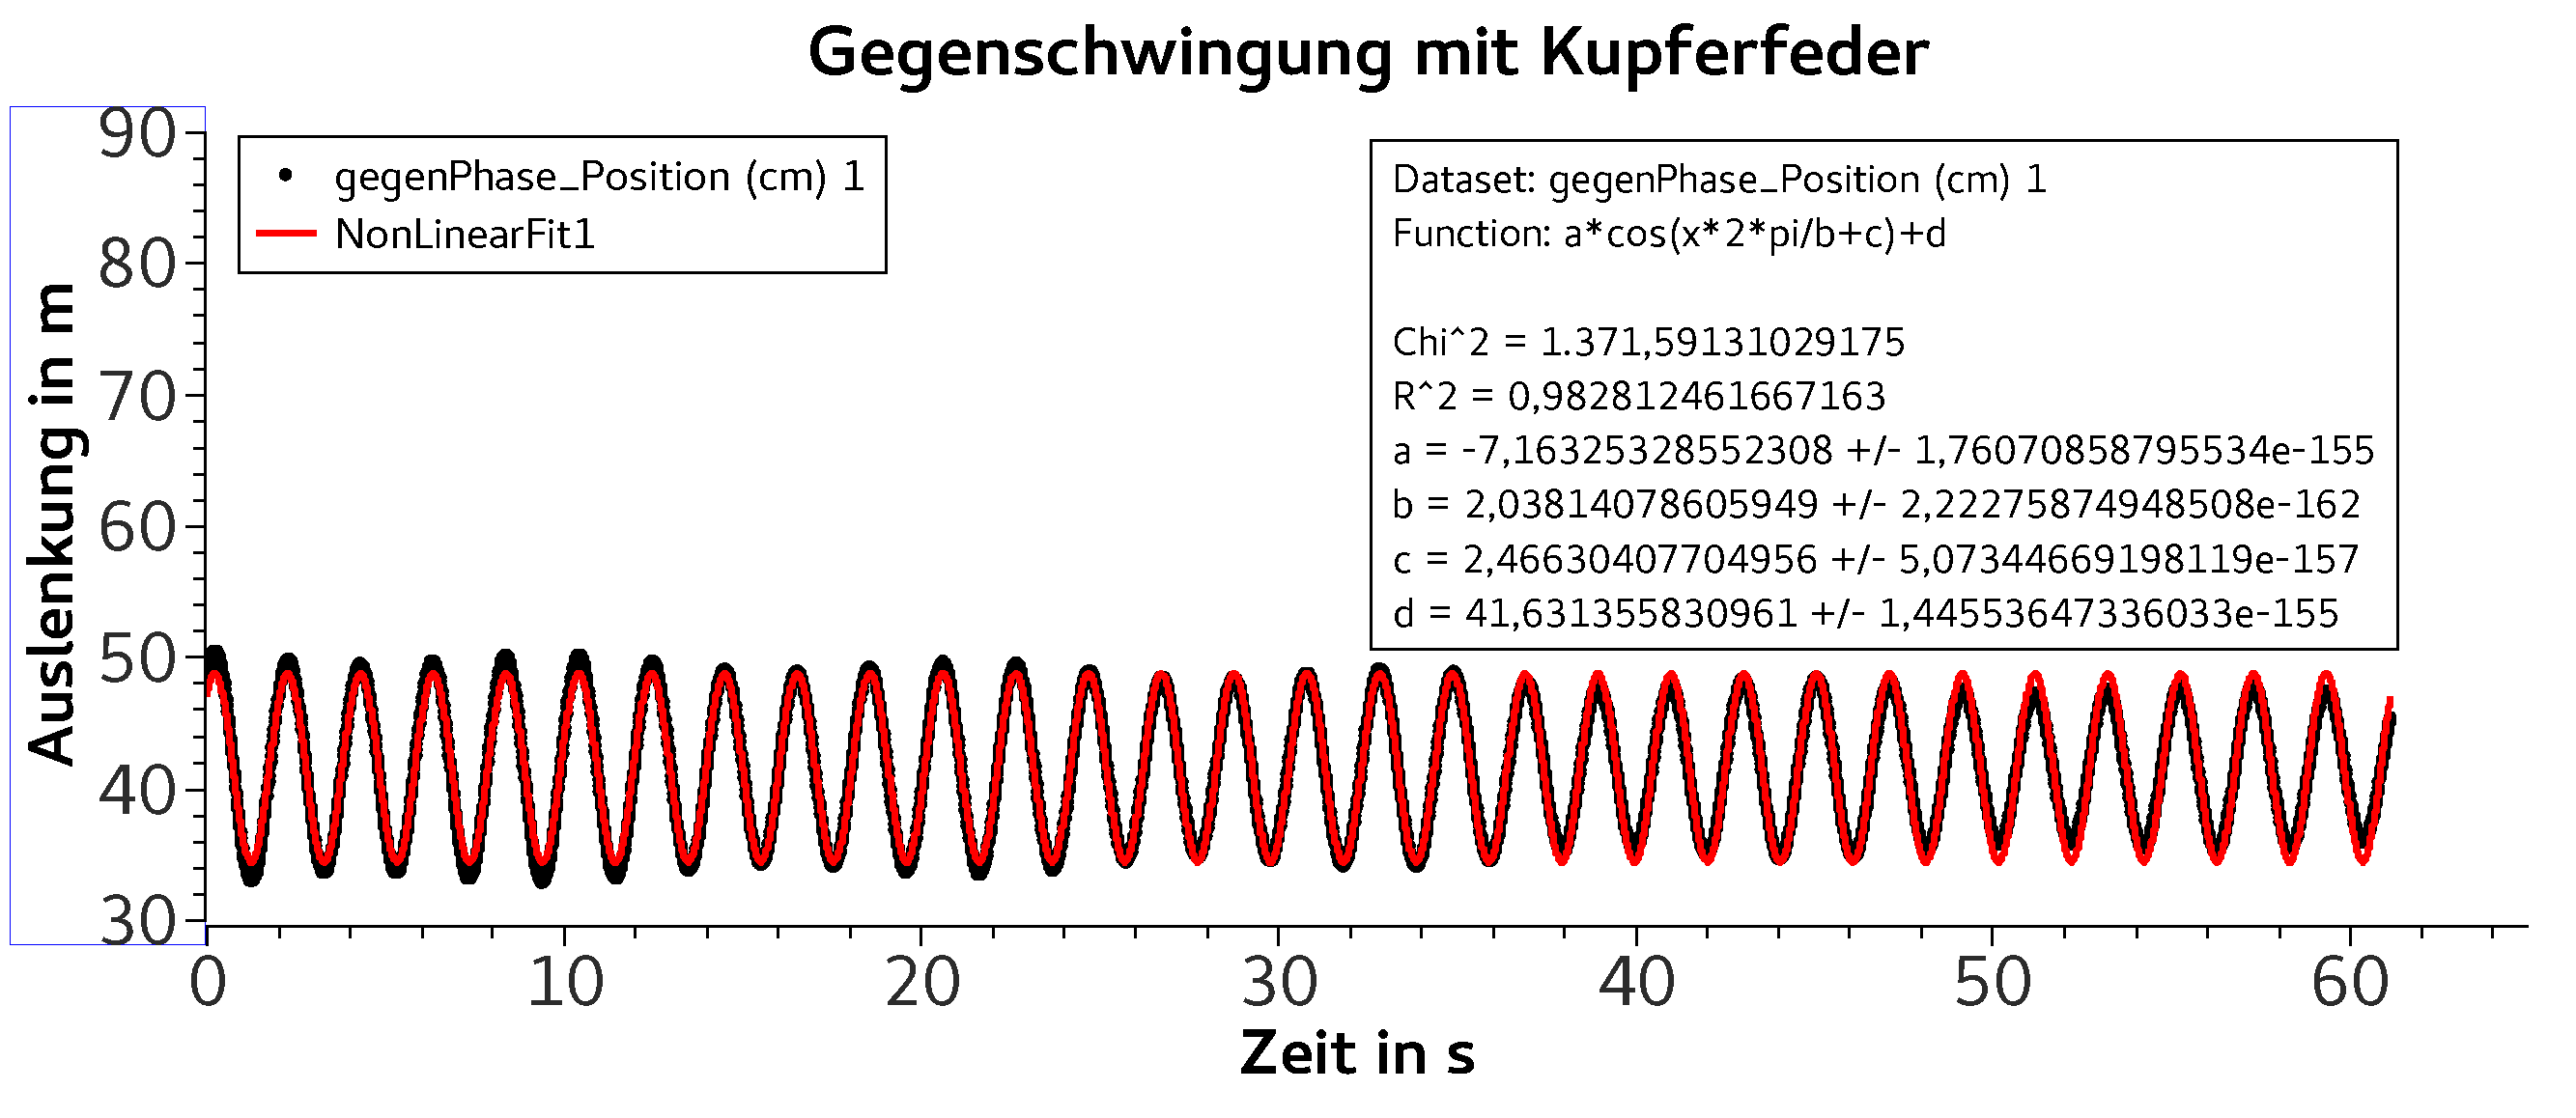
\includegraphics[width=1\textwidth]{KupferGegenschwingung}
		\centering
		\caption{Gegenschwingung mit Kupferfeder.}
		\label{KupferGegenschwingung}
		\centering
	\end{figure}

	\subsubsection*{Edelstahl}
	Aus \cref{EdelstahlGegenschwingung} lässt sich $T_\text{geg,St}$ aus den Parametern des Fits ablesen. Der Parameter $b$ ist die Schwingdauer und beträgt \SI{1,7518}{s}.
	\begin{figure}[H]
		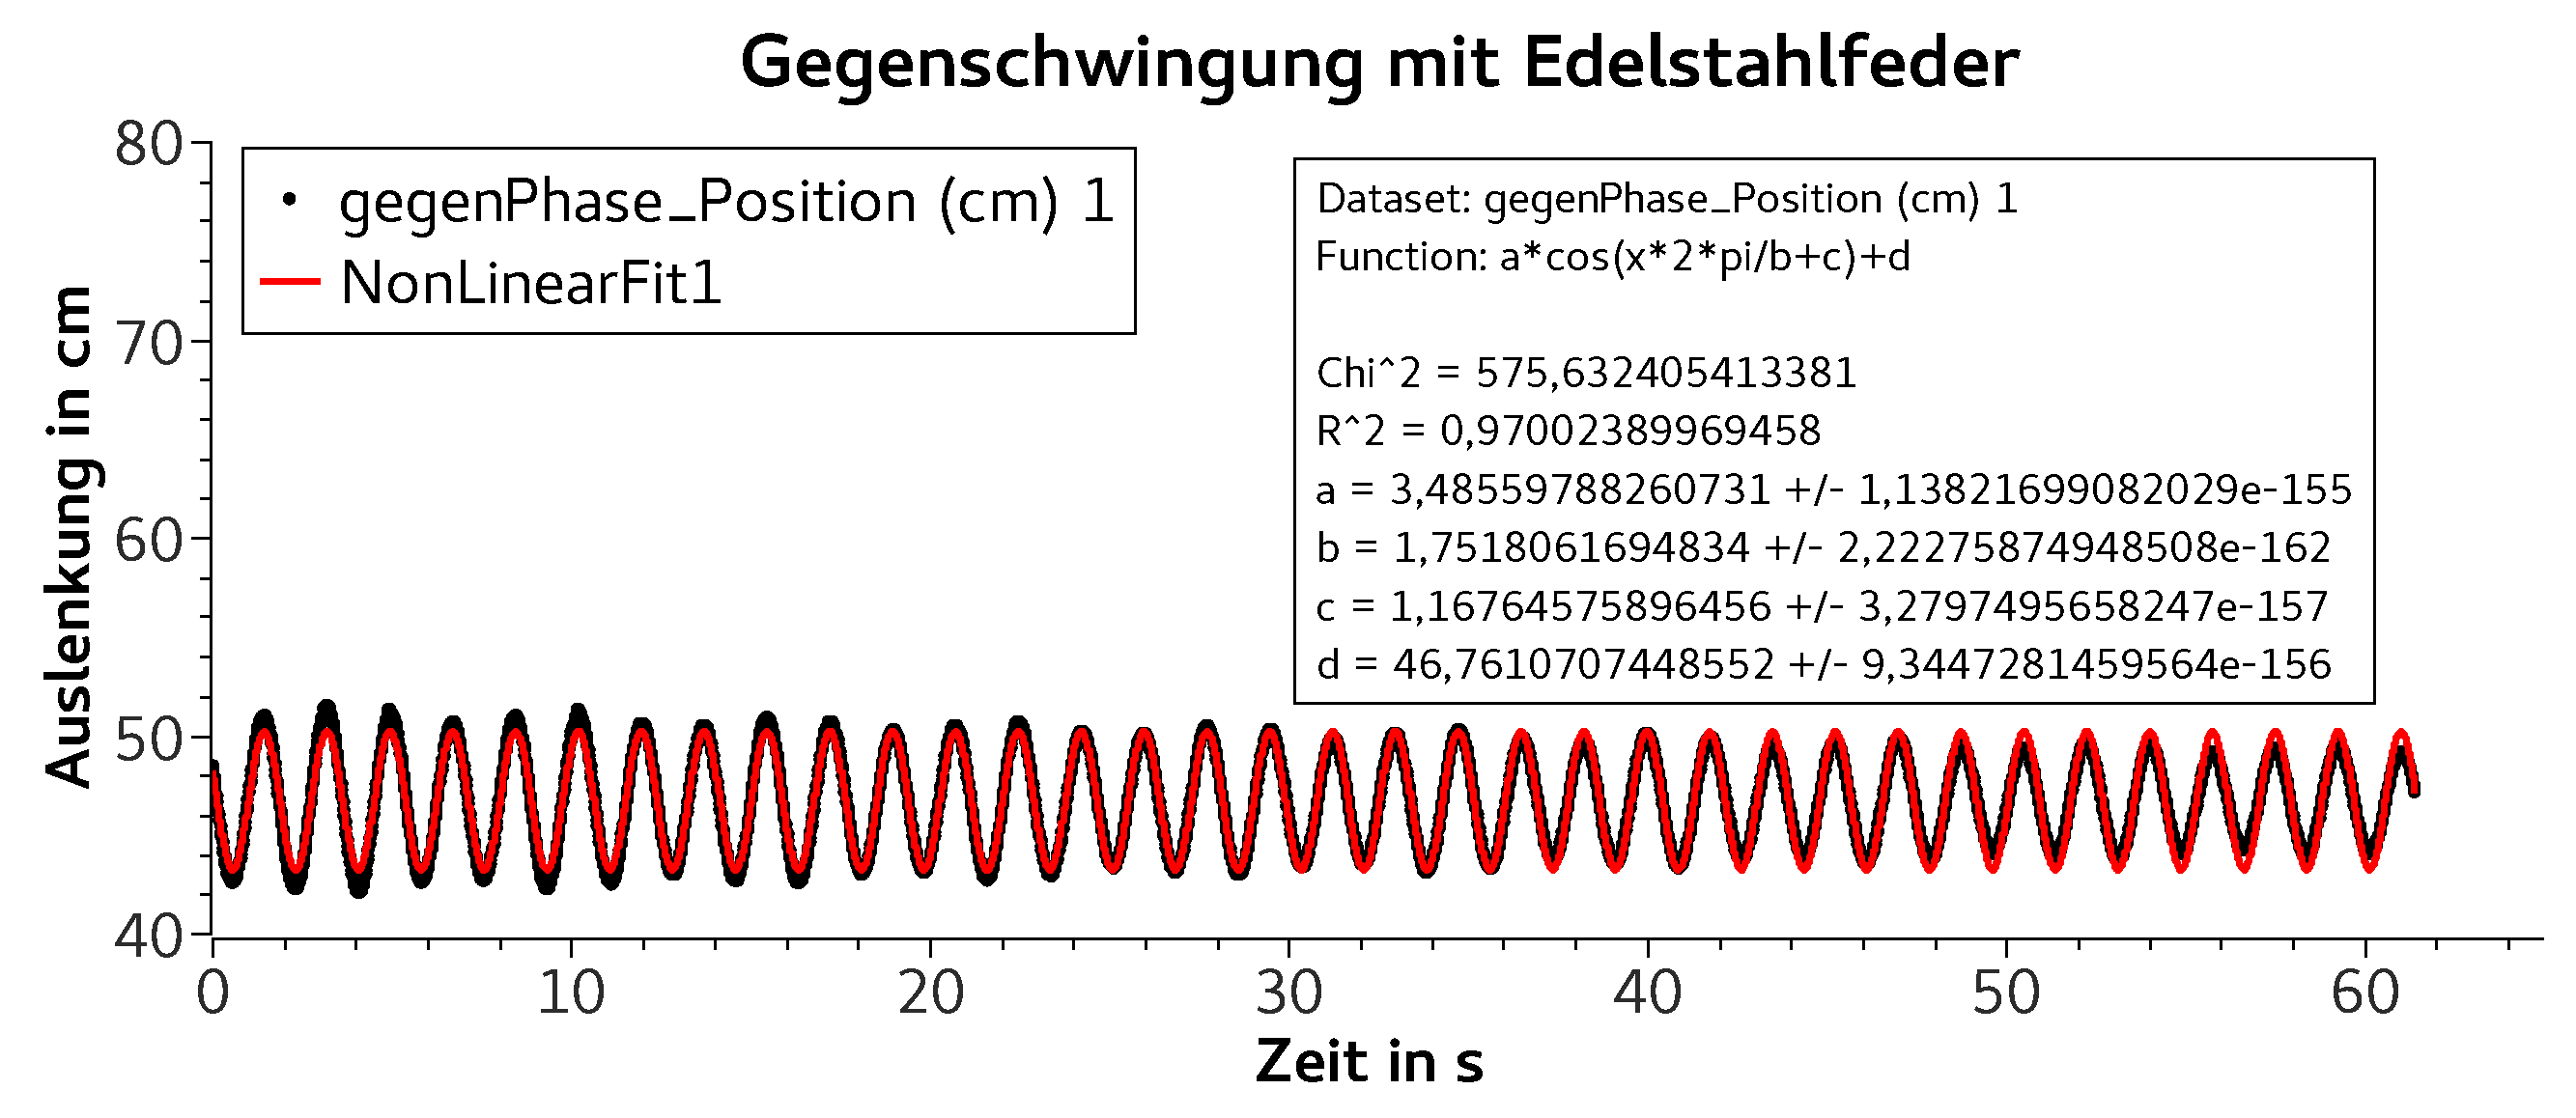
\includegraphics[width=1\textwidth]{EdelstahlGegenschwingung}
		\centering
		\caption{Gegenschwingung mit Edelstahlfeder.}
		\label{EdelstahlGegenschwingung}
		\centering
	\end{figure}



	\subsubsection{Schwebungen des gekoppelten Systems}

	\subsubsection*{Kupfer}
	Aus \cref{KupferSchwebung} lässt sich $T_\text{S,Cu}$ aus den Parametern des Fits ablesen. Der Parameter $c$ gibt die Winkelgeschwindigkeit der Schwebung an. Folglich ist die Schwebungsdauer $T_\text{S,Cu} = \frac{2\pi}{\omega} = \SI{23,484}{s}$.
	\begin{figure}[H]
		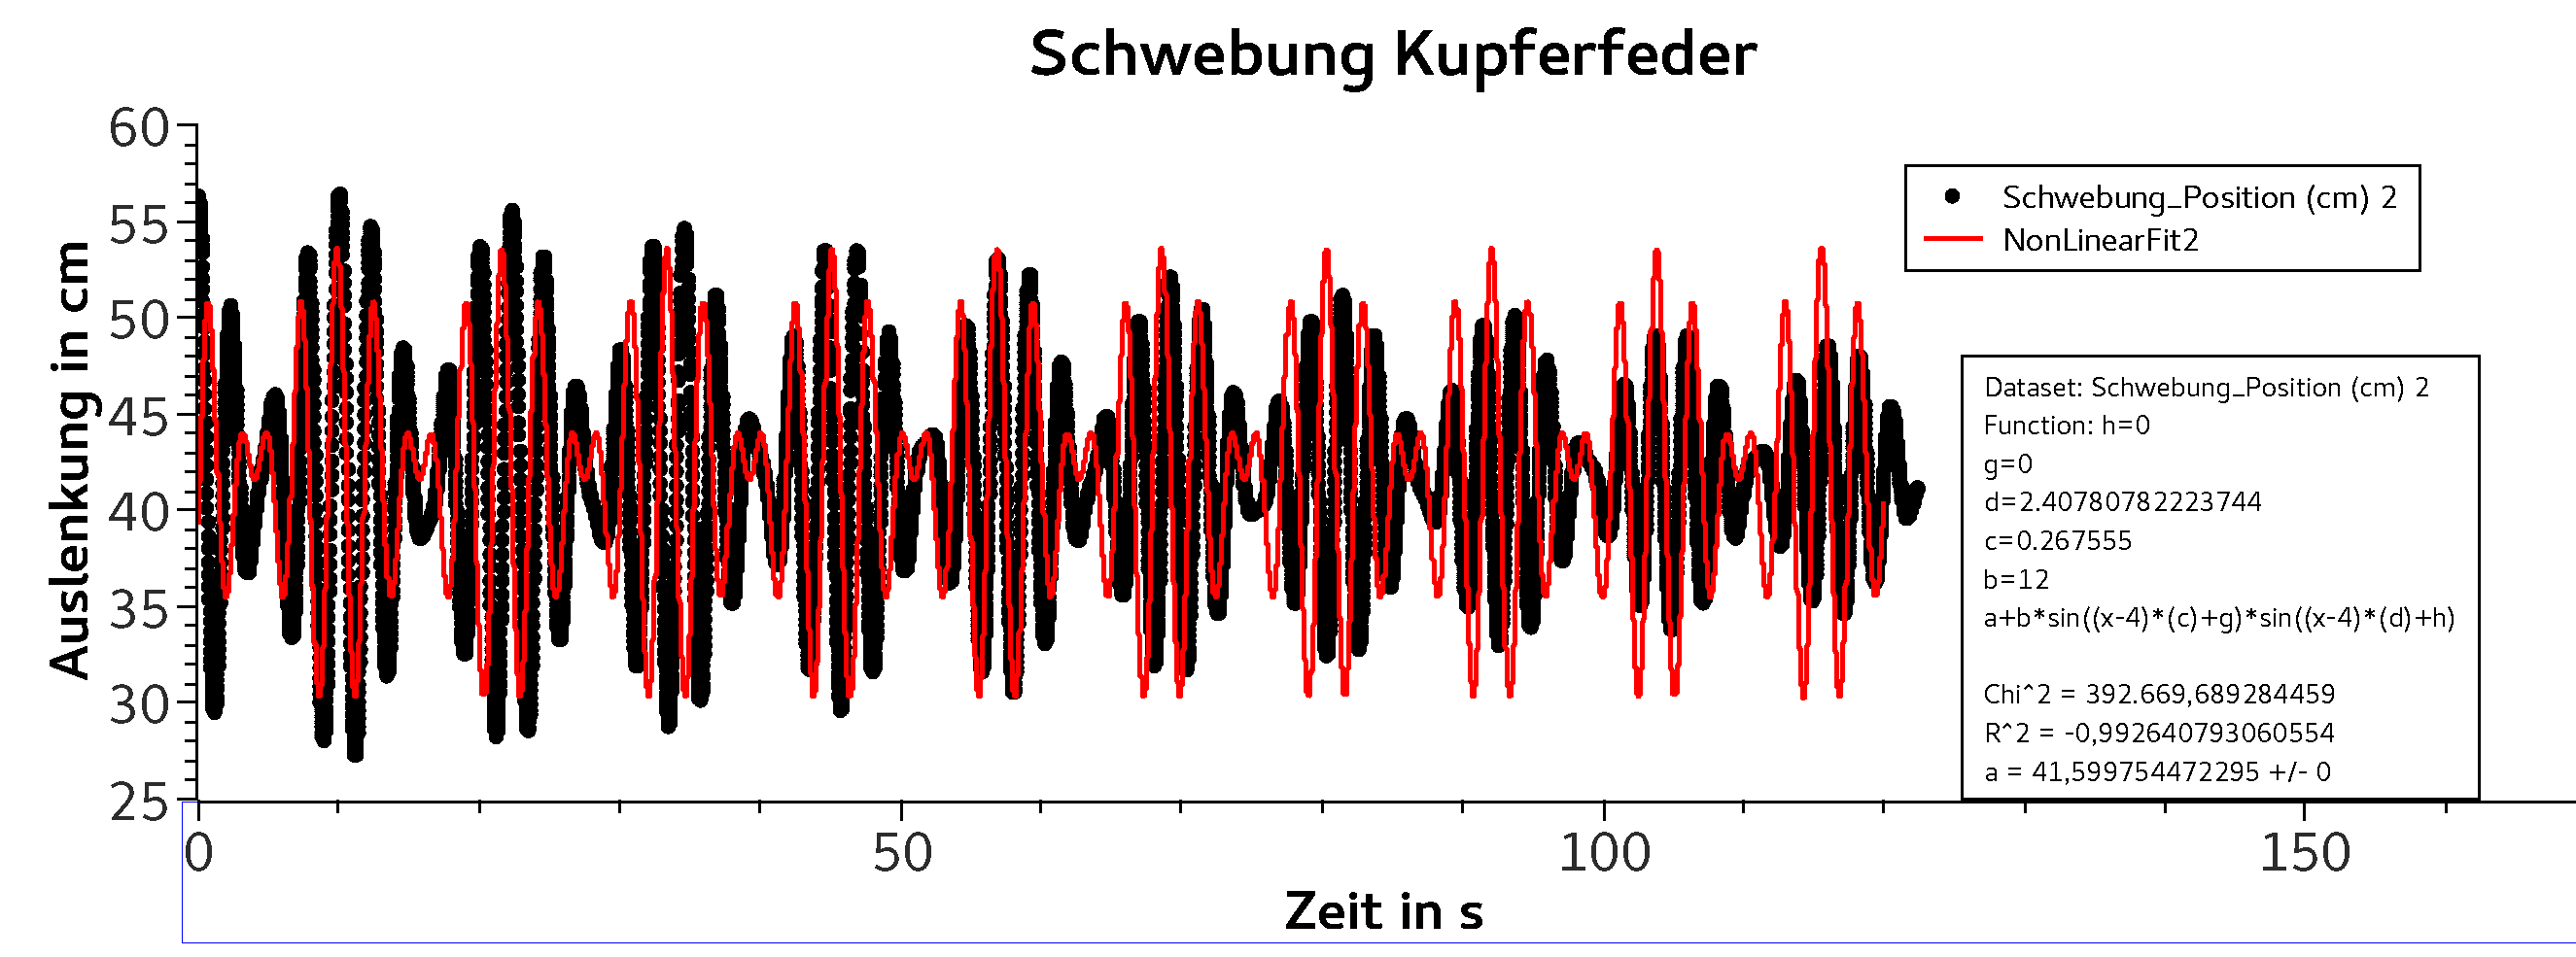
\includegraphics[width=1\textwidth]{KupferSchwebung}
		\centering
		\caption{Schwebungen mit Kupferfeder.}
		\label{KupferSchwebung}
		\centering
	\end{figure}

	\subsubsection*{Edelstahl}
	Aus \cref{EdelstahlSchwebung} lässt sich $T_\text{S,St}$ aus den Parametern des Fits ablesen. Der Parameter $c$ gibt die Winkelgeschwindigkeit der Schwebung an. Folglich ist die Schwebungsdauer $T_\text{S,St} = \frac{2\pi}{\omega} = \SI{12,323}{s}$.
	\begin{figure}[H]
		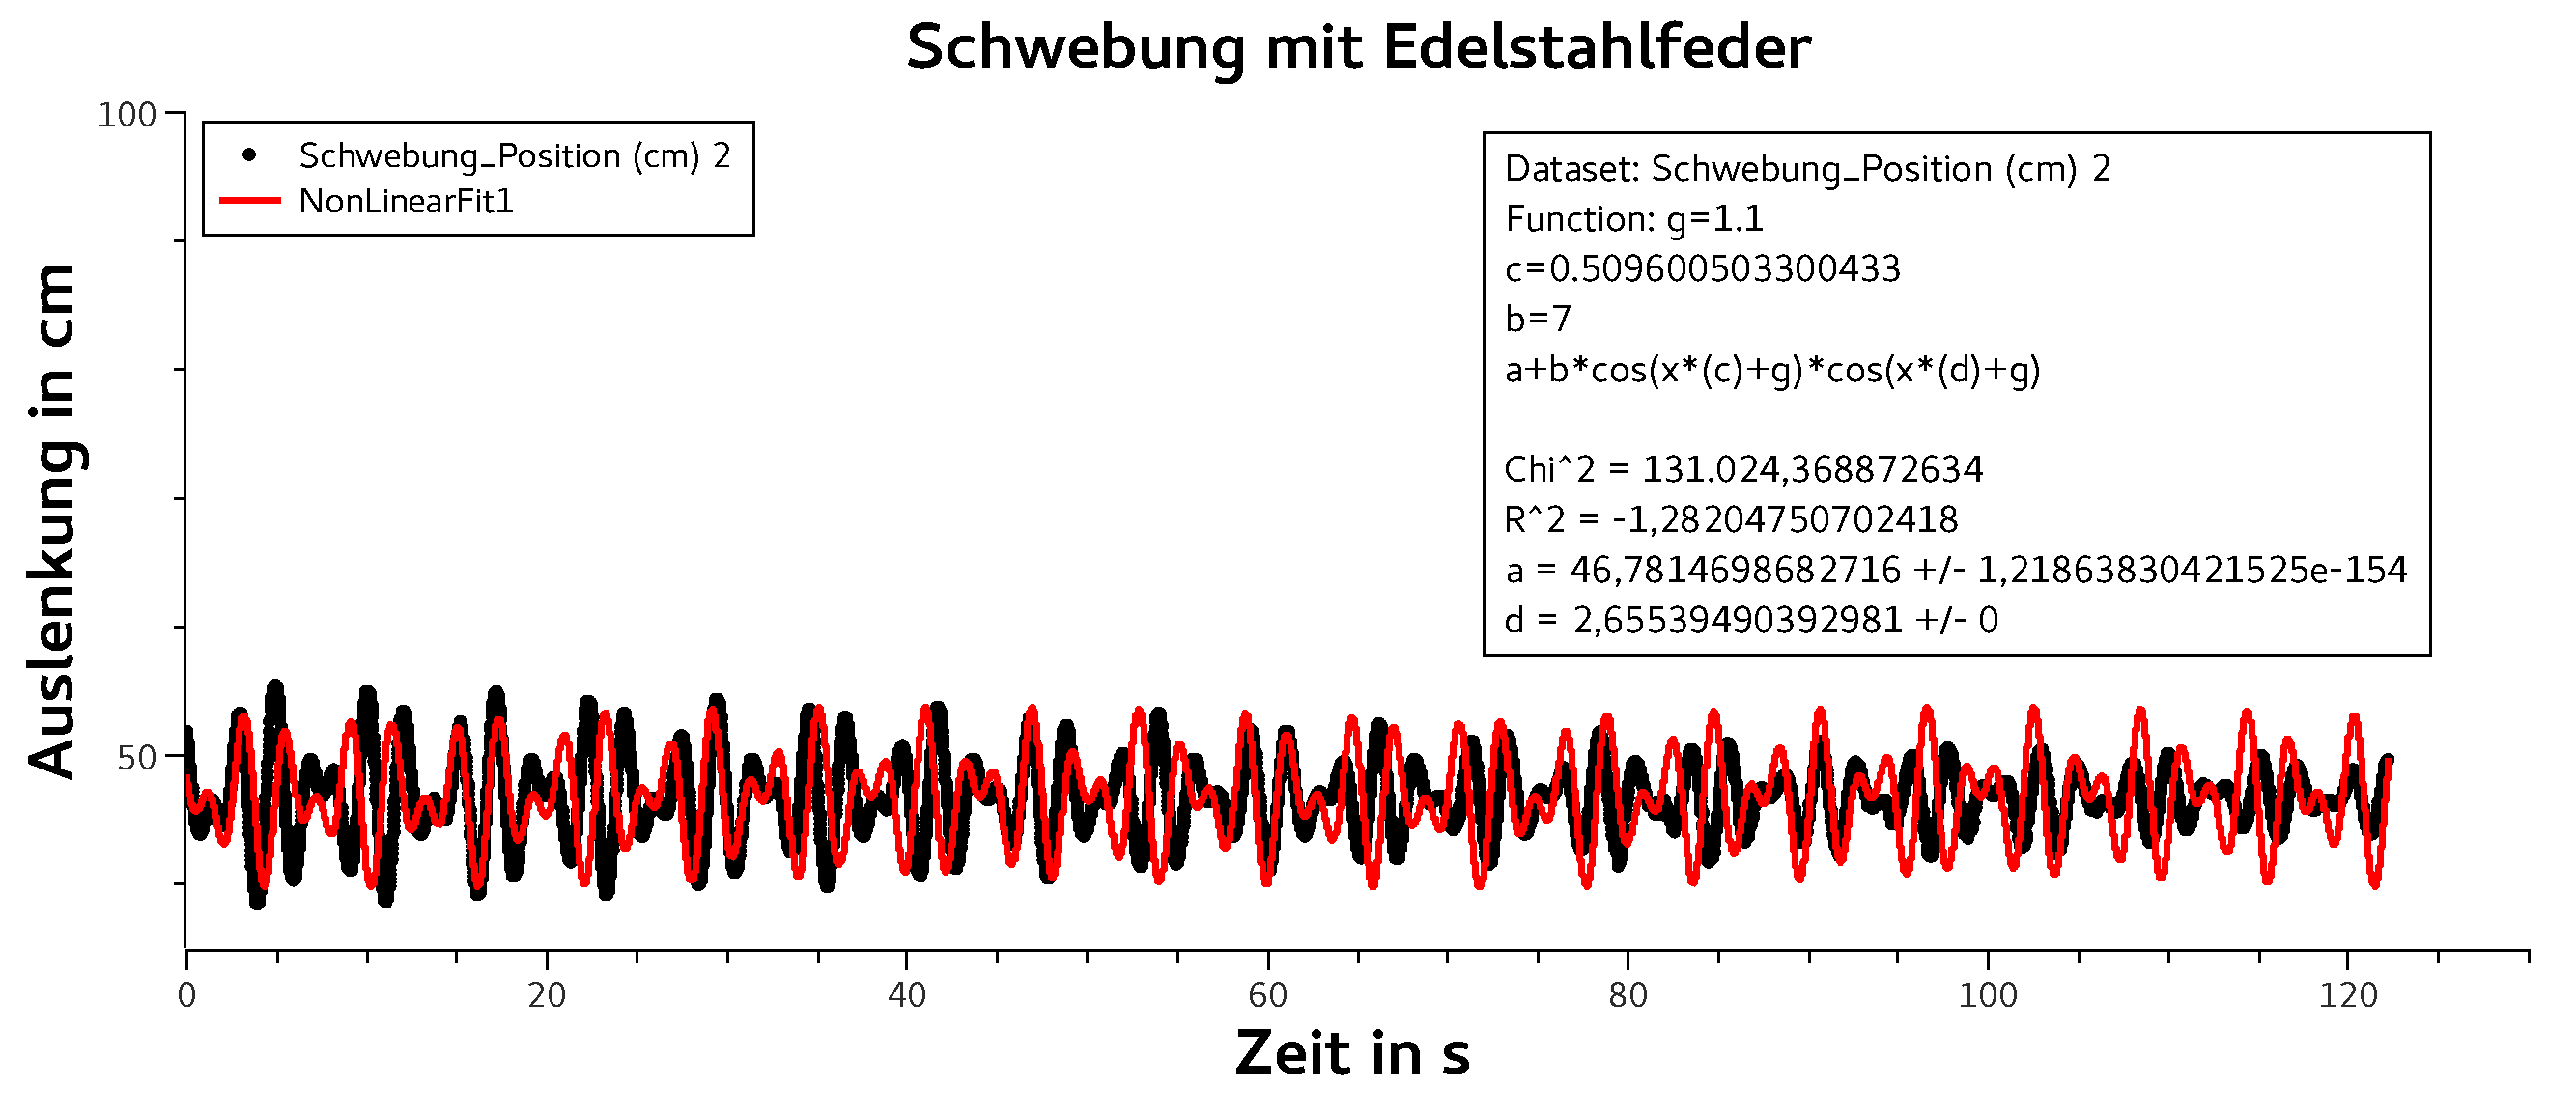
\includegraphics[width=1\textwidth]{EdelstahlSchwebung}
		\centering
		\caption{Schwebungen mit Edelstahlfeder.}
		\label{EdelstahlSchwebung}
		\centering
	\end{figure}

	\subsubsection{Vergleich der Schwingdauern}
	\label{Vergleich der Schwingdauern}
	Die Fehler der Fitalgorithmen für die Schwingdauern sind immer kleiner $10^{-100}$ und folglich vernachlässigbar. Da jedoch verschiedene Fehler beim Experiment durch beispielweise die Kleinwinkelnäherung, die beim Berechnen der Bewegungsgleichung des Pendels angewendet wurde, auftreten können, wurde die Unsicherheit der Schwingdauer der Fitalgorithmen großzügig mit \SI{0,001}{s} abgeschätzt.
	\begin{table}[H]
	\centering
	\begin{tabular}{ l | c | c | c |}
		& Kupfer & Edelstahl  \\ \hline
		$T_\text{gl} $ &$\SI{2,4645 \pm 0,001}{s}$&$\SI{2,4437 \pm 0,001}{s}$\\  
		$T_\text{geg} $ &$\SI{2,0381 \pm 0,001}{s}$&$\SI{1,7518 \pm 0,001}{s}$\\  
		$T_\text{S} $ &$\SI{23,484 \pm 0,001}{s}$&$\SI{12,323 \pm 0,001}{s}$\\  \hline
	\end{tabular}
	\caption{Messwerte gekoppelter Pendel}
	\end{table}
	Auffällig ist der Zusammenhang
	\begin{equation}
		T_0 >  T_\text{gl,Cu} > T_\text{gl,St}.
	\end{equation}
	Der Theorie nach sollte jedoch gelten 
	\begin{equation}
		T_0 =  T_\text{gl,Cu} = T_\text{gl,St}.
	\end{equation}
	Es ist anzunehmen, dass die veränderte Schwingdauer durch das Einbinden der Feder in das System verursacht wurde. Im idealen Fall würde die Ruhelänge der Feder dem Abstand der Pendel, wenn sie nicht schwingen, entsprechen. Beim Koppeln der Pendel änderte sich die Ruhelage der Pendel. Dies hat zur Folge, dass der Abstand der Pendel nicht mehr für alle Zeiten gleich ist, wenn sie mit derselben Frequenz schwingen.
	\newline
	\noindent{}In der Anleitung war diese Formel für die Schwebungsdauer gegeben:
	\begin{equation}
		T_S = \frac{4\pi}{\omega_{geg}-\omega_{gl}} = \frac{2}{\frac{1}{T_{geg}} - \frac{1}{T_{gl}}}
	\end{equation}
	\begin{align}
		u(T_S) &= \sqrt{\left(\frac{\partial T_S}{\partial T_{geg}}u(T_{geg}) \right)^2 + \left(\frac{\partial T_S}{\partial T_{gl}}u(T_{gl}) \right)^2 } \\
		&= u(T_{gl})\sqrt{\left(\frac{2T_{gl}^2}{(T_{geg}-T_{gl})^2} \right)^2 + \left(\frac{-2T_{geg}^2}{(T_{geg}-T_{gl})^2} \right)^2 } \\
		&= \frac{2u(T_{gl})}{(T_{geg}-T_{gl})^2}\sqrt{(T_{gl})^4 + (T_{geg})^4 } 
	\end{align}
	\begin{table}[H]
	\centering
	\begin{tabular}{ l | c | c | c |}
		& Kupfer & Edelstahl  \\ \hline
		$T_\text{S,Rechnung}$ &$\SI{23,560 \pm 0,081}{s}$&$\SI{12,374 \pm 0,028}{s}$\\  \hline
		$T_\text{S,Messung} $ &$\SI{23,484 \pm 0,001}{s}$&$\SI{12,323 \pm 0,001}{s}$\\  \hline
	\end{tabular}
	\caption{Schwebungsdauern berechnet aus den Schwingdauern der Gleich- und Gegenschwingung}
	\end{table}
	Die Unsicherheitsintervalle der Kupferfeder überschneiden sich, aber die der Edelstahlfeder weisen einen deutlichen Unterschied auf. Grund dafür ist wahrscheinlich, dass die Fitfunktion der Edelstahlfeder eine zu große Abweichung von den Messpunkten hat.
	\begin{table}[H]
	\centering
	\begin{tabular}{ l | c | c | c |}
		& Kupfer & Edelstahl  \\ \hline
		$R^2$ &$\SI{0,99264}{}$&$\SI{1,2820}{}$\\  \hline
	\end{tabular}
	\caption{$R^2$ für die Fitkurven der Schwebungen}
	\end{table}

	\subsubsection{Dynamische Bestimmung des Kopplungsgrads}
	Setzt man die ermittelten Schwingdauern in
	\begin{equation}
		k = \frac{T_{gl}^2-T_{geg}^2}{T_{gl}^2+T_{geg}^2}
	\end{equation}
	\begin{align}
		u(k) &= \sqrt{\left(\frac{\partial k}{\partial T_{geg}}u(T_{geg}) \right)^2 + \left(\frac{\partial k}{\partial T_{gl}}u(T_{gl}) \right)^2 } \\
		&=                         ...\\
		&= \frac{4u(T_{gl})T_{geg}T_{gl}}{(T_{geg}^2+T_{gl}^2)^\frac{3}{2}}
	\end{align}
	ein, ergeben sich folgende Kopplungsgrade:
	\begin{table}[H]
	\centering
	\begin{tabular}{ l | c | c | c |}
		& Kupfer & Edelstahl  \\ \hline
		$k$ &$\SI{0,1877 \pm 0,0006}{}$&$\SI{0,3211 \pm 0,0006}{}$\\  \hline
	\end{tabular}
	\caption{Kopplungsgrade aus den Schwingdauern}
	\end{table}
	\noindent{}Die dynamisch ermittelten Kopplungsgrade liegen innerhalb der Unsicherheit der statisch ermittelten Kopplungsgrade (\cref{TabelleStatischKopplungsgrad}).


	\subsubsection{Relative Frequenzaufspaltung}
	Die relative Frequenzaufspaltung lässt sich mittels der gegebenen Formeln bestimmen.
	\begin{equation}
		\frac{\Delta\omega}{\omega_0} = \frac{\omega_{geg}-\omega_{gl}}{\omega_{gl}} = 2\frac{T_{gl}}{T_S}
	\end{equation}
	Wobei sich die Unsicherheit aus folgender Formel ergibt.
	\begin{align}
		u(k) &= \sqrt{\left(\frac{\partial \frac{\Delta\omega}{\omega_0} }{\partial T_{S}}u(T_{S}) \right)^2 + \left(\frac{\partial \frac{\Delta\omega}{\omega_0} }{\partial T_{gl}}u(T_{gl}) \right)^2 } \\
			&= 2ku(T_{gl}) \sqrt{\left(\frac{1}{T_S}\right)^2 + \left(\frac{1}{T_{gl}}\right)^2 }
	\end{align}

	\begin{table}[H]
	\centering
	\begin{tabular}{ l | c | c | c |}
		& Kupfer & Edelstahl  \\ \hline
		$\frac{\Delta\omega}{\omega_0}  $ &$\SI{0,2099 \pm 0,0002}{}$&$\SI{0,3966 \pm 0,0003}{}$\\  \hline
	\end{tabular}
	\caption{relative Frequenzaufspaltungen}
	\end{table}

	\subsubsection{Diskussion der Näherung}
	Zum Berechnen der relative Frequenzaufspaltung ist außerdem die folgende Formel aufgeführt
	\begin{equation}
		\frac{\Delta\omega}{\omega_0} = \sqrt{\frac{1+k}{1-k}} -1 
	\end{equation}
	und deren Näherung
	\begin{equation}
		\frac{\Delta\omega}{\omega_0} = k + \frac{k^2}{2} + \frac{k^3}{2} + O(k^4)
	\end{equation}
	Die Unsicherheit von unserem statischen Kopplungsgrad $k$ beträgt 0,006. Für die Formel ergibt sich die Unsicherheit
	\begin{equation}
		u\left({\frac{\Delta\omega}{\omega_0}}\right) = \left| \frac{\partial (\frac{\Delta\omega}{\omega_0})}{\partial k} u(k)\right| = \left|\frac{u(k)}{(k-1)^2\sqrt{\frac{1+k}{1-k}}} \right|
	\end{equation}
	und für die Näherung
	\begin{equation}
		u\left({\frac{\Delta\omega}{\omega_0}}\right) = \left| \frac{\partial (\frac{\Delta\omega}{\omega_0})}{\partial k} u(k)\right| = \left| u(k)(1+k+\frac{3}{2}k^2) \right|
	\end{equation}

	\begin{table}[H]
	\centering
	\begin{tabular}{ l | c | c | c |}
		& Kupfer & Edelstahl  \\ \hline
		Aus der Kopplungsformel   &$\SI{0,2171 \pm 0,0076}{}$&$\SI{0,3779 \pm 0,0091}{}$\\  \hline
		Aus der Kopplungsnäherung   &$\SI{0,2165 \pm 0,0075}{}$&$\SI{0,3729 \pm 0,0087}{}$\\  \hline
		Aus den Schwingdauern   &$\SI{0,2099 \pm 0,0002}{}$&$\SI{0,3966 \pm 0,0003}{}$\\  \hline
	\end{tabular}
	\caption{relative Frequenzaufspaltungen}
	\end{table}
	\noindent{}Die relative Abweichung des Wertes der Näherung zu dem der Formel beträgt für die Edelstahlfeder ca. \SI{~1}{\%} und für die Kupferfeder ca. \SI{0,2}{\%}.
	Es ist wieder eine Abweichung bei den Werten der Edelstahlfeder ersichtlich. Diese Varianz tratt bereits beim Vergleichen der Schwebungsdauern auf (siehe \cref{Vergleich der Schwingdauern}).


	
	\subsubsection*{Unsicherheiten}
	Der Ultraschallsensor misst lediglich den Abstand in der Horizontalen, das Pendel dagegen rotiert in einer Ebene. Da bei diesem Versuch der Fokus auf den Schwingdauern lag, ist der Fehler der Schwingungsamplitude irrelevant. Des Weiteren muss man davon ausgehen, dass das Verarbeiten der Daten des Sensors Zeit beansprucht. Da diese jedoch jeden Messpunkt gleichermaßen zeitlich verschiebt, kann auch dieser Fehler für eine Betrachtung der Schwingdauern vernachlässigt werden.
	
	


	\subsection{Doppelpendel}
	Das Doppelpendel schwingt sehr chaotisch, d.h. es ergeben sich auch bei einer nur sehr kleinen Änderung der Anfangsbedingungen deutlich andere Bahnen und auch eine längere Beobachtung der Bahn erlaubt keine Vorhersage auf deren zukünftigen Verlauf. Allerdings konnten wir zwei stabile Schwingungszustände beobachten, jedoch nur für ca. 5 Perioden. Danach ergaben sich minimal phasenverschobene Schwingungen. Bei einer der stabilen Schwingungen haben beide Pendel immer in die selbe Richtung gezeigt. Die andere zeichnet sich da durch aus, dass die Pendel immer den entgegengesetzten Winkel zur Vertikalen haben. Um diese stabilen Schwingungszustände präziser, und somit länger anhaltend, umzusetzen, wäre eine Apparatur, die die Startauslenkung der Pendelarme kontrolliert und einen exakt gleichzeitigen Start der Schwingung beider Arme ermöglicht.%TODO mehr

	\section{Schlussfolgerung}
	%TODO machen
	Da wir die Feder nur ca. \SI{10}{cm} über den Gewichten der Pendel befestigt hatten, ergab sich für unsere Messungen ein hoher Kopplungsgrad. Entsprechend sind unsere relativen Frequenzaufspaltungen hoch und und die Schwebungsdauern klein.  Dies machte die Auswertung ungenauer. Des Weiteren hätte sich mit geringerem Kopplungsgrad auch die Frequenzen der Gleichschwingungen weniger von der Eigenfrequenz des einzelnen Pendels unterschieden.
	Die Taylorentwicklung 3. Ordnung erwies sich bei unseren Kopplungsgraden als eine gute Approximation der Formel für die relative Frequenzaufspaltung mit ca. \SI{1}{\%} Abweichung.
	Gleichermaßen wie bei den gekoppelten Fadenpendeln gab es auch beim Doppelpendel zwei stabile Schwingungen. Deutlich unterschieden sich die Pendel, wenn keiner der Spezialfälle vorlag. Die gekoppelten Pendel oszillierten noch erkennbar mit der Überlagerung von zwei Schwingungen. Das Doppelpendel dagegen schwang chaotisch und ein periodischer Zusammenhang war nict ersichtlich.
	
	%\printbibliography
\end{document}
